%%%%%%%%%%%%%%%%%%%%%%%%%%%%%%%%%%%%%%%%%
% University/School Laboratory Report
% LaTeX Template
% Version 3.1 (25/3/14)
%
% This template has been downloaded from:
% http://www.LaTeXTemplates.com
%
% Original author:
% Linux and Unix Users Group at Virginia Tech Wiki 
% (https://vtluug.org/wiki/Example_LaTeX_chem_lab_report)
%
% License:
% CC BY-NC-SA 3.0 (http://creativecommons.org/licenses/by-nc-sa/3.0/)
%
%%%%%%%%%%%%%%%%%%%%%%%%%%%%%%%%%%%%%%%%%

%----------------------------------------------------------------------------------------
%	PACKAGES AND DOCUMENT CONFIGURATIONS
%----------------------------------------------------------------------------------------

\documentclass{article}

\usepackage[version=3]{mhchem} % Package for chemical equation typesetting
\usepackage{siunitx} % Provides the \SI{}{} and \si{} command for typesetting SI units
\usepackage{graphicx} % Required for the inclusion of images
\usepackage{natbib} % Required to change bibliography style to APA
\usepackage{amsmath} % Required for some math elements 
\usepackage{caption}
\usepackage{subcaption}
\usepackage{listings}
\usepackage{color}
 
\definecolor{codegreen}{rgb}{0,0.6,0}
\definecolor{codegray}{rgb}{0.5,0.5,0.5}
\definecolor{codepurple}{rgb}{0.58,0,0.82}
\definecolor{backcolour}{rgb}{0.95,0.95,0.92}
 
\lstdefinestyle{mystyle}{
    backgroundcolor=\color{backcolour},   
    commentstyle=\color{codegreen},
    keywordstyle=\color{codepurple},
    numberstyle=\tiny\color{codegray},
    stringstyle=\color{codepurple},
    basicstyle=\footnotesize,
    breakatwhitespace=false,         
    breaklines=true,                 
    captionpos=b,                    
    keepspaces=true,                 
    numbers=left,                    
    numbersep=5pt,                  
    showspaces=false,                
    showstringspaces=false,
    showtabs=false,                  
    tabsize=2
}
\lstset{style=mystyle}

\setlength\parindent{0pt} % Removes all indentation from paragraphs

\renewcommand{\labelenumi}{\alph{enumi}.} % Make numbering in the enumerate environment by letter rather than number (e.g. section 6)

\newcommand\tab[1][0.5cm]{\hspace*{#1}}

%\usepackage{times} % Uncomment to use the Times New Roman font

%----------------------------------------------------------------------------------------
%	DOCUMENT INFORMATION
%----------------------------------------------------------------------------------------

\title{COMP 429/529: Project 2} % Title

\author{Berkay \textsc{Barlas}} % Author name

\date{\today} % Date for the report

\begin{document}

\maketitle % Insert the title, author and date

\begin{center}
\begin{tabular}{l r}
Date Performed: & March 17, 2019 \\ % Date the experiment was performed
Instructor: & Didem Unat % Instructor/supervisor
\end{tabular}
\end{center}

% If you wish to include an abstract, uncomment the lines below
% \begin{abstract}
% Abstract text
% \end{abstract}

%----------------------------------------------------------------------------------------
%	SECTION 1
%----------------------------------------------------------------------------------------

\tab In this assignment I implemented MPI and OpenMP versions
on top of given serial version for Cardiac Electrophysiology Simulation and conducted experiments. 
\\ \tab  To compile all the necessary files run \"make cardiacsim \&\& make serial \&\& make openmp\"
\newline
In this assignment I have completed
\begin{itemize}
    \item 1D MPI version of Cardiac Electrophysiology Simulation
    \item 2D MPI version of Cardiac Electrophysiology Simulation
    \item 2D MPI+OpenMP version of Cardiac Electrophysiology Simulation
    \item Performance Studies for Part a, b, c, d, e
\end{itemize}

\section{Implementation}
\subsection{MPI Implementation}
\tab 
Cardiac Electrophysiology simulator solves system of Ordinary Differential Equations (ODEs) together with Partial Differential Equations (PDEs). 
\begin{itemize}
\item Initial data used in this equations are created by master process ,then, it is distributed to other processes using MPI\_Scatterv. 
\begin{lstlisting}[language=C]
    MPI_Scatterv(s_src[0], sendcounts, displs, box, 
    s_dst[0], x*y, MPI_DOUBLE, 0, MPI_COMM_WORLD);
\end{lstlisting}
\item After the processes recieve the sub parts of data they only calculate their own part. 
\begin{lstlisting}[language=C]
    simulate(my_E, my_E_prev, my_R, alpha, x_size,  y_size, kk, dt, a, epsilon, M1, M2, b, x_pos, y_pos, px, py);
\end{lstlisting}
\item These calculations requires some data which changes every iteration from neighbour processes, therefore, ghost cell implementation is needed. All processes use Non\-Blocking Messages to Communicate to their neighbours. They wait for their send and recieve requests with MPI\_wait().
\begin{lstlisting}[language=C]
    /// send and recieve ghost cells to and from neighbor processes 
      // top side send&recieve
      if(y_pos != 0){
        MPI_Irecv(my_E_prev[0], x_size+2, MPI_DOUBLE, upperRank, BOTTOMTAG, MPI_COMM_WORLD, &reqs[requestCount++]);
        MPI_Isend(my_E_prev[1], x_size+2, MPI_DOUBLE, upperRank, UPPERTAG, MPI_COMM_WORLD, &reqs[requestCount++]); 
      }
      // bottom side send&recieve
      if(y_pos != ((P - 1) / px) ) {
        MPI_Irecv(my_E_prev[y_size+1], x_size+2, MPI_DOUBLE, bottomRank, UPPERTAG, MPI_COMM_WORLD, &reqs[requestCount++]);
        MPI_Isend(my_E_prev[y_size], x_size+2, MPI_DOUBLE, bottomRank, BOTTOMTAG, MPI_COMM_WORLD, &reqs[requestCount++]); 
      }
      // left side send&recieve
      if(x_pos != 0 ) {
        int i; 
        for(i = 0; i < y_size; i++) {
        leftSend[i] = my_E_prev[i+1][1]; 
        }
        MPI_Irecv(&left[0], y_size, MPI_DOUBLE, rightRank, LEFTTAG, MPI_COMM_WORLD, &reqs[requestCount++]);
        MPI_Isend(&leftSend[0], y_size, MPI_DOUBLE, rightRank, RIGHTTAG, MPI_COMM_WORLD, &reqs[requestCount++]); 
      }
      // right side send&recieve
      if(x_pos != ((P-1) % px)) {
        int i; 
        for(i = 0; i < y_size; i++) {
        rightSend[i] = my_E_prev[i+1][x_size];
        }
        MPI_Irecv(&right[0], y_size, MPI_DOUBLE, leftRank, RIGHTTAG, MPI_COMM_WORLD, &reqs[requestCount++]);
        MPI_Isend(&rightSend[0], y_size, MPI_DOUBLE, leftRank, LEFTTAG, MPI_COMM_WORLD, &reqs[requestCount++]);   
      } 
      //
      MPI_Waitall(requestCount, reqs, status);
      // left side
      int i;
      if(x_pos != 0 ) {
      for(i = 0; i < y_size; i++) {
        my_E_prev[i+1][0] = left[i];
      }
      }
      // right side 
      if(x_pos != ((P-1) % px)) {
        for(i = 0; i < y_size; i++) {
          my_E_prev[i+1][x_size+1] = right[i];
        }
      }
\end{lstlisting}
\item Since the data transferred from left and right sides are not sequential in memory, they are send to and recieved from array buffers.
\begin{lstlisting}[language=C]
double *leftSend, *rightSend, *left, *right; 

right = (double*) malloc(y_size * sizeof(double));
left = (double*) malloc(y_size * sizeof(double));
rightSend = (double*) malloc(y_size * sizeof(double));
leftSend = (double*) malloc(y_size * sizeof(double));
\end{lstlisting}
\item Then, the sub data in different processes are collected by master processes using MPI\_Gatherv.
\item To handle the case when the processor geometry doesn’t evenly divide the size of the mesh. I increased the mesh size.
\end{itemize}

\subsection{OpenMP Implementation}
\tab I Added OpenMP parallelism within an MPI process to support hybrid parallelism with MPI+OpenMP.\\
\tab I defined parallel section where the 3 equations solved. I used \#pragma omp for collapse(2) because the nested loops are data indepedent.
\\ \tab \textbf{Example execution:}\\ mpirun -np 1 -bind-to socket -map-by socket ./cardiacsim-openmp -n 1024 -o 2 -t 100 -x 1 -y 1

\begin{lstlisting}[language=C]
#pragma omp parallel 
  {
    #pragma omp for collapse(2)
    for (j=1; j<=m; j++){
      for (i=1; i<=n; i++) {
	E[j][i] = E_prev[j][i]+alpha*(E_prev[j][i+1]+E_prev[j][i-1]-4*E_prev[j][i]+E_prev[j+1][i]+E_prev[j-1][i]);
      }
    }
    
    /* 
     * Solve the ODE, advancing excitation and recovery to the
     *     next timtestep
     */
    #pragma omp for collapse(2)
    for (j=1; j<=m; j++){
      for (i=1; i<=n; i++)
	E[j][i] = E[j][i] -dt*(kk* E[j][i]*(E[j][i] - a)*(E[j][i]-1)+ E[j][i] *R[j][i]);
    }
    
    #pragma omp for collapse(2)
    for (j=1; j<=m; j++){
      for (i=1; i<=n; i++)
	R[j][i] = R[j][i] + dt*(epsilon+M1* R[j][i]/( E[j][i]+M2))*(-R[j][i]-kk* E[j][i]*(E[j][i]-b-1));
    }
  }
\end{lstlisting}

%----------------------------------------------------------------------------------------
%	SECTION Studies
%----------------------------------------------------------------------------------------
\newpage

\section{Studies}
\subsection{Part A: Strong Scaling}
\begin{description}
    \item[Optimal processor geometry: 1 x 32] \hfill 
    \item[Single Processor Gflops Rate: ] 6.04524  \hfill
    \item[Original Serial Code Gflops Rate: ] 6.00341 \hfill
    
\end{description}

\textbf{Results}
\begin{figure}[!htb]
    \centering
    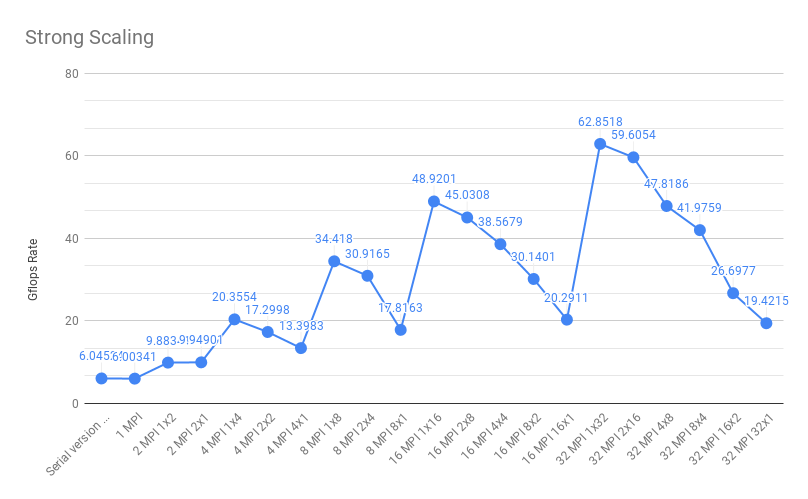
\includegraphics[width=1\linewidth]{./img/Strong-Scaling.png}
    \caption{Strong Scaling results}
\end{figure}   


\textbf{Observation}
\\ \tab There is a slight performance difference between my MPI code with single processor and original code. This difference might caused by MPI initialization. The difference is small because there is not communication between processors.
\\ \tab Increasing the number of processes increase the performance and 1D horizontal data partitioning performs better than other geometries.

\newpage


\subsection{PART B: Strong Scaling with ntasks-per-node=16}
	
\textbf{Results}
\begin{figure}[!htb]
    \centering
    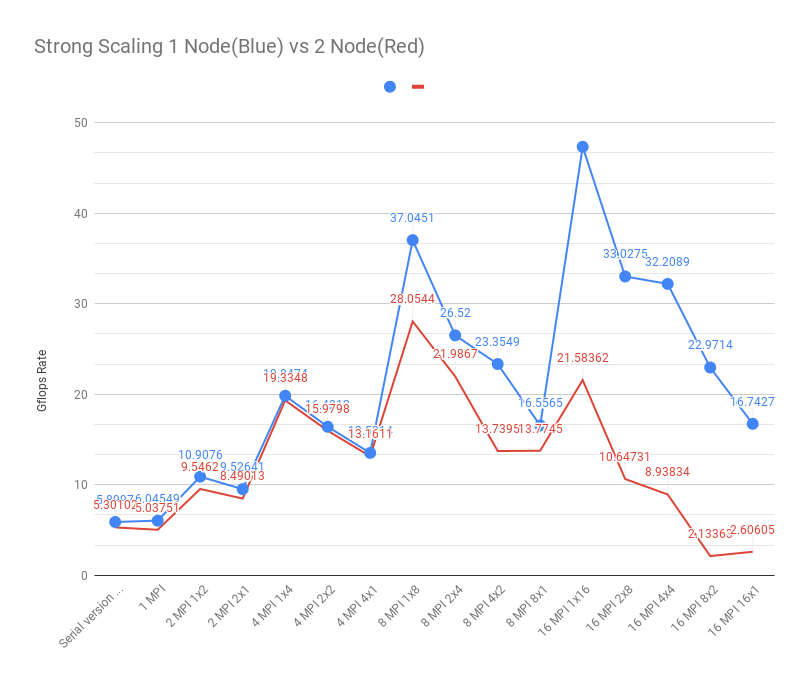
\includegraphics[width=1\linewidth]{./img/1vs2.png}
    \caption{Strong Scaling results with Single and Dual nodes}
\end{figure}  
\\ 
\textbf{Comparison the single node performance with dual node performance}
The single node performance is better than dual performance nearly for every geometry. Also, the performance difference is increases with increasing number of MPI processes. This might be caused by communication overhead between processes in different nodes.

\newpage

\subsection{Part C: Disabling Communication}
\tab In this part, I calculated Communication overhead by disabling Communication. When the no\_comm variable is equal to 1 the communication is disabling. 
\begin{lstlisting}[language=C]
    if(no_comm == 0) {

    // Communication codes

    }
\end{lstlisting}
\begin{equation*}
    Communication Overhead  = (1 - \frac{Execution Time with No Communication}{Execution Time with Communication} * 100)
    %\begin{center}\ce{}\end{center}
\end{equation*}

\begin{figure}[!htb]
    \centering
    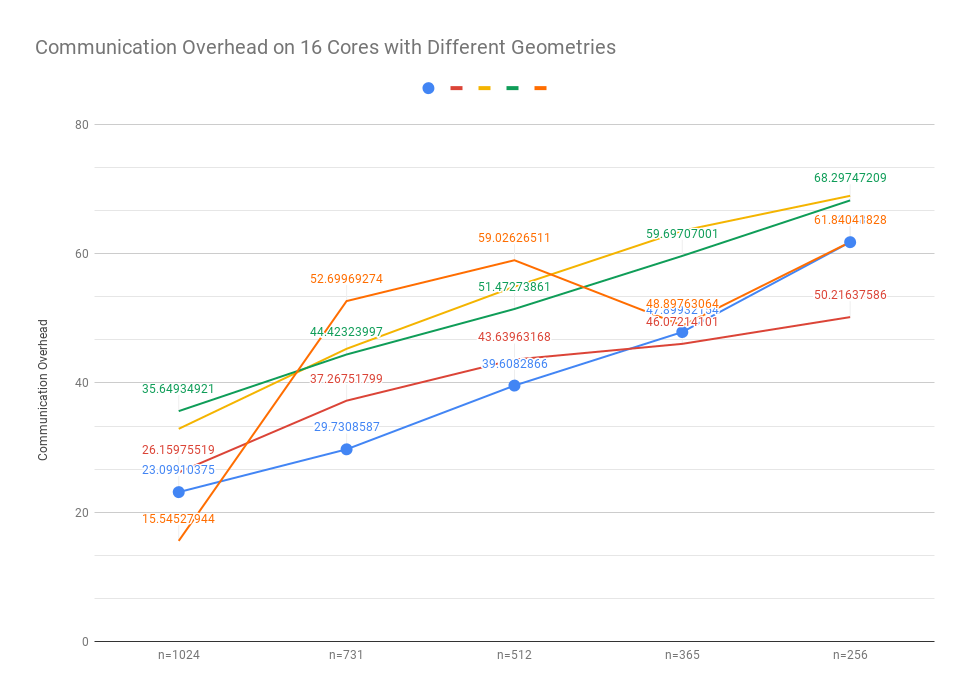
\includegraphics[width=1\linewidth]{./img/comOverhead.png}
    \caption{Communication Overhead results with different geometries on 16 cores. \textbf{Blue=1x16
    Red=2x8 Yellow=4x4 Green=8x2 Orange=16x1}}
\end{figure}  

\textbf{Observation}
\\ \tab The communication overhead increases as the total amount of data decrease because the calculation / communication ratio decrease for every core.
\\ \tab Also, the communication overhead results are higher than what I expected this might happened because of the change in calculations. A better approach would be creating the no\_comm system such that the processes would make same calculations with communication enabled system.
\newpage
\subsection{Part D: Single and Dual Node Performance with OpenMP}
In this study, 1D geometry used for MPI+OpenMP hybrid parallelism.

\begin{description}
    \item[Which combination of MPI+OpenMP is the fastest?: ] \hfill \\ 8 MPI Processes + 4 OpenMP Thread is the fastest
\end{description}

\begin{figure}[!htb]
    \centering
    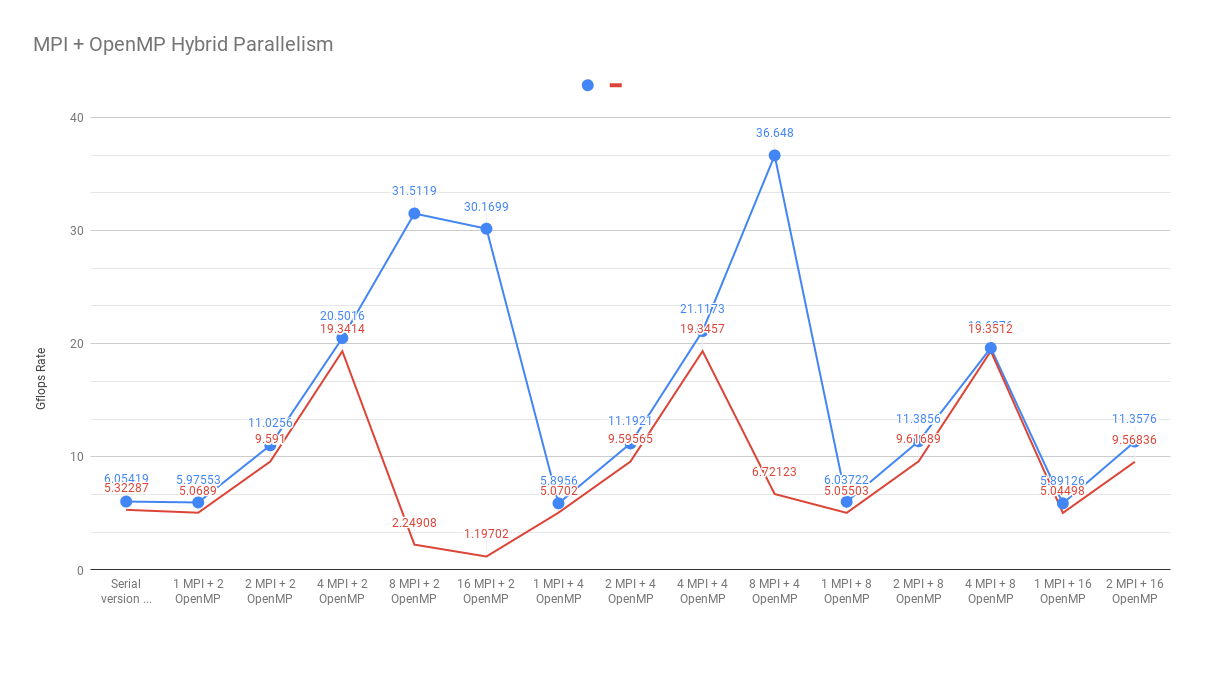
\includegraphics[width=1\linewidth]{./img/mpi+openmp.png}
    \caption{Single(Blue) and Dual(Red) node performance study}
\end{figure}  

\textbf{Observations}
\\ \tab The single node performance is also better than dual performance nearly for every geometry in this study with OpenMP. This might be caused by communication overhead between processes in different nodes. The 2 nodes might be run on different machines, this might create an unequal systems which gives unstable results.
\\ \tab The performance difference is also effected by the thread number. When the number of MPI cores increases the performance decrease due to OpenMP parallelization overhead.
\\ 
\newpage

\begin{figure}[!htb]
    \centering
    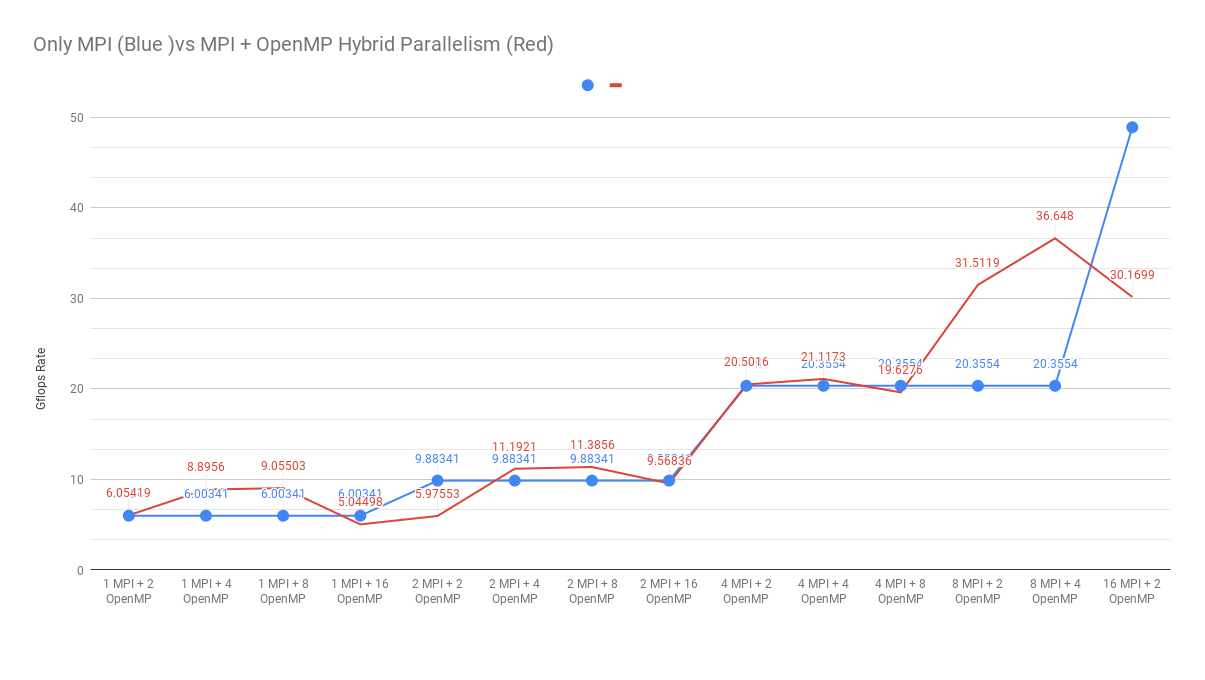
\includegraphics[width=1\linewidth]{./img/mpivsopenmp.png}
    \caption{MPI Only(Blue) vs MPI + OpenMP performance comparison on single node}
\end{figure} 

\textbf{Observations}
 \\ \tab With the same number of MPI processes, Number of OpenMP thread increases performance until some point ,then, decrease the performance. 
 \\ \tab Number of MPI cores affect performance more than Number of OpenMP Threads. Overall performance increases as the MPI core number increase.

\newpage

\subsection{Part E: Weak Scaling Study}
In this study, I conduct a weak scaling to observe the running time while successively doubling the number of cores, starting at P=1 core with N = 256 ending at 32 cores on two nodes. I calculated t such that iteration number is equals 10000.
\begin{figure}[!htb]
    \centering
    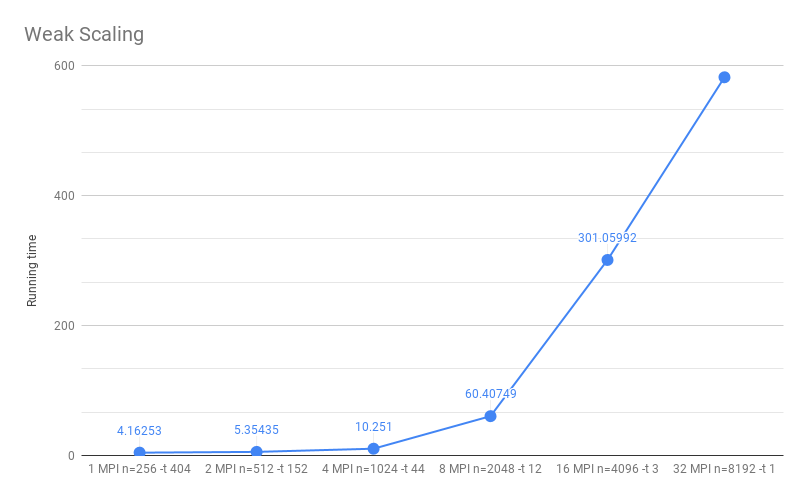
\includegraphics[width=1\linewidth]{./img/Weak-Scaling.png}
    \caption{Results for the weak scaling}
\end{figure}
\\ \tab Eventhough, number of cores and N values are growing linearly, the running time increases polynomially because the complexity of system is N\^2.  

%----------------------------------------------------------------------------------------
%	SECTION 6
%----------------------------------------------------------------------------------------

\section{Formulas Used}

\begin{enumerate}
\begin{item}
    \emph{Communication Overhead} 
    \begin{equation*}
    Communication Overhead  = (1 - \frac{Execution Time with No Communication}{Execution Time with Communication} * 100)
    %\begin{center}\ce{}\end{center}
    \end{equation*}
\end{item}

\end{enumerate}




\end{document}